\section{Descrizione singoli componenti}
\subsection{Package mytalk.client.iView}{
\subsubsection{Package mytalk.client.iView.iAdministrator}{

	\begin{figure}[h!tbp]
		\centering
		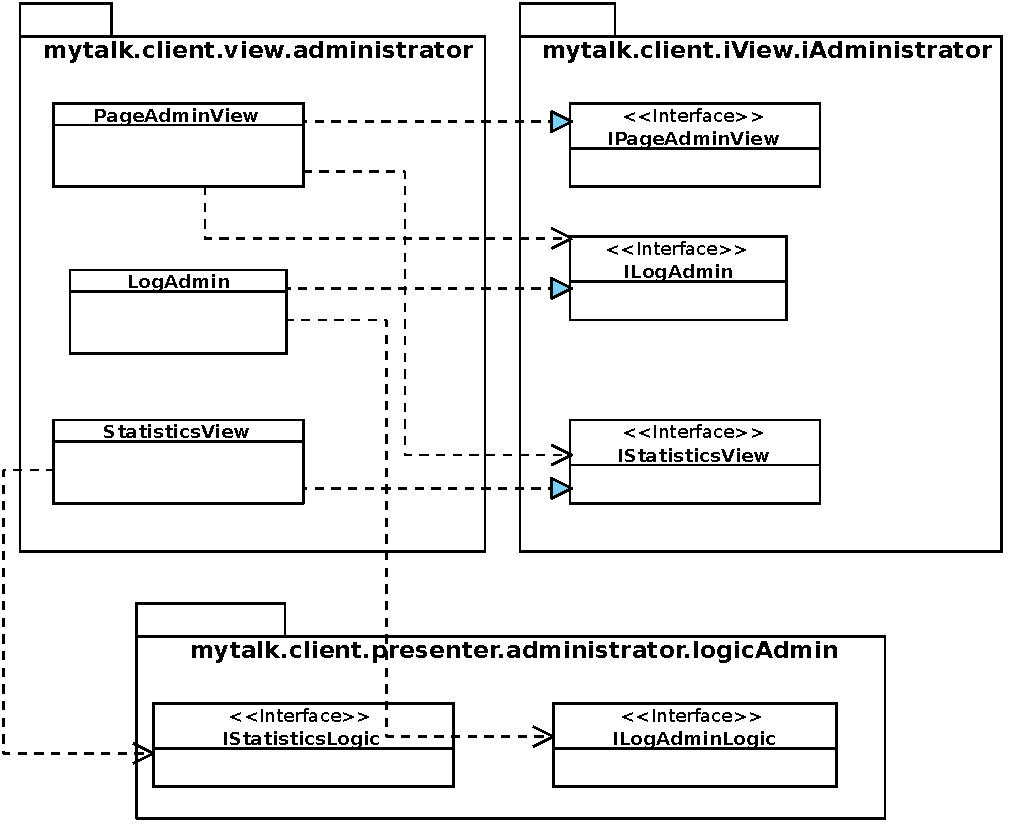
\includegraphics[scale=0.80]{\docsImg dia/MyTalk-View-Admin.pdf}
		\caption{Diagramma delle classi che illustra la View amministratore.}
	\end{figure}

%interfacce
\paragraph{IPageAdminView}{
	\begin{itemize}
		\item [] \textbf{Nome:} \texttt{IPageAdminView}
		\item [] \textbf{Tipo:} interface
		\item [] \textbf{Package:} \texttt{mytalk.client.iView.iAdministrator}
		\item [] \textbf{Descrizione:}{ interfaccia che permette di gestire gli oggetti che compongono la GUI\g~ dell'amministratore.}
	\end{itemize}
}
\paragraph{ILogAdmin}{
	\begin{itemize}
		\item [] \textbf{Nome:} \texttt{ILogAdmin}
		\item [] \textbf{Tipo:} interface
		\item [] \textbf{Package:} \texttt{mytalk.client.iView.iAdministrator}
		\item [] \textbf{Descrizione:}{ interfaccia che permette di richiedere, da parte dell'utente amministratore, l'accesso al servizio o alla sua terminazione. Le classi che implementano questa interfaccia hanno il compito di raccogliere ed inoltrare al sottosistema Presenter i dati di accesso, nel caso di un login, e distruggere la sessione utente amministratore in caso di logout.}
	\end{itemize}
}
\paragraph{IStatisticView}{
	\begin{itemize}
		\item [] \textbf{Nome:} \texttt{IStatisticView}
		\item [] \textbf{Tipo:} interface
		\item [] \textbf{Package:} \texttt{mytalk.client.iView.iAdministrator}
		\item [] \textbf{Descrizione:}{ interfaccia che permette, agli oggetti che la implementano, di inviare messaggi al Presenter che permettono il recupero e il filtraggio delle statistiche.}
	\end{itemize}
}
}


\subsubsection{Package mytalk.client.iView.iUser}{

	\begin{figure}[h!tbp]
		\centering
		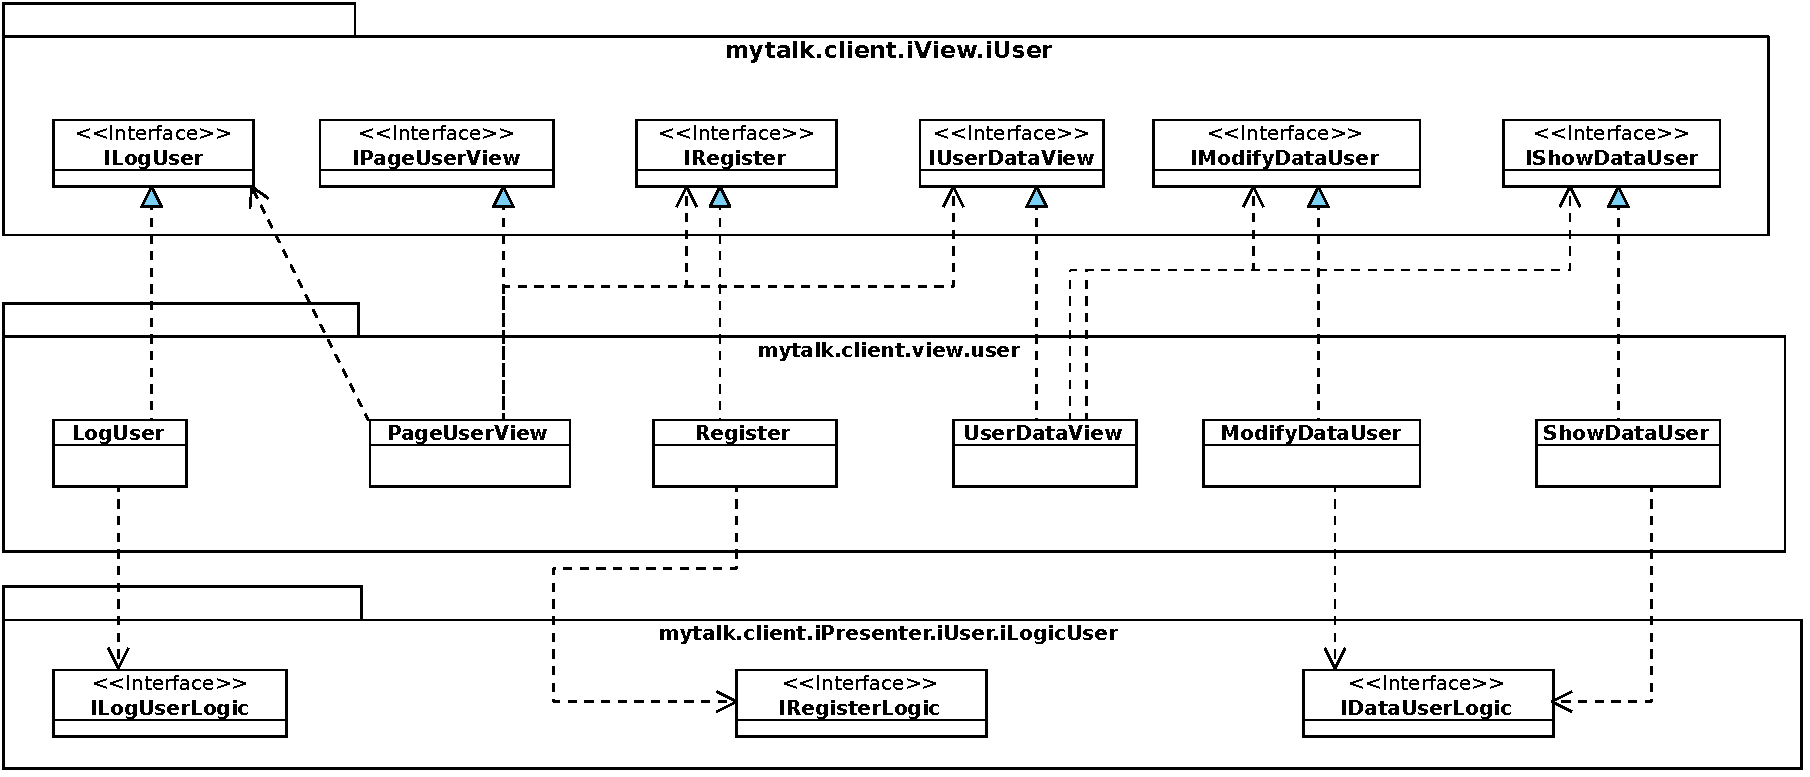
\includegraphics[scale=0.55]{\docsImg dia/MyTalk-View-User.pdf}
		\caption{Diagramma delle classi che illustra la View utente per le operazioni di login e gestione dati.}
	\end{figure}
	\newpage
	\begin{figure}[h!tbp]
		\centering
		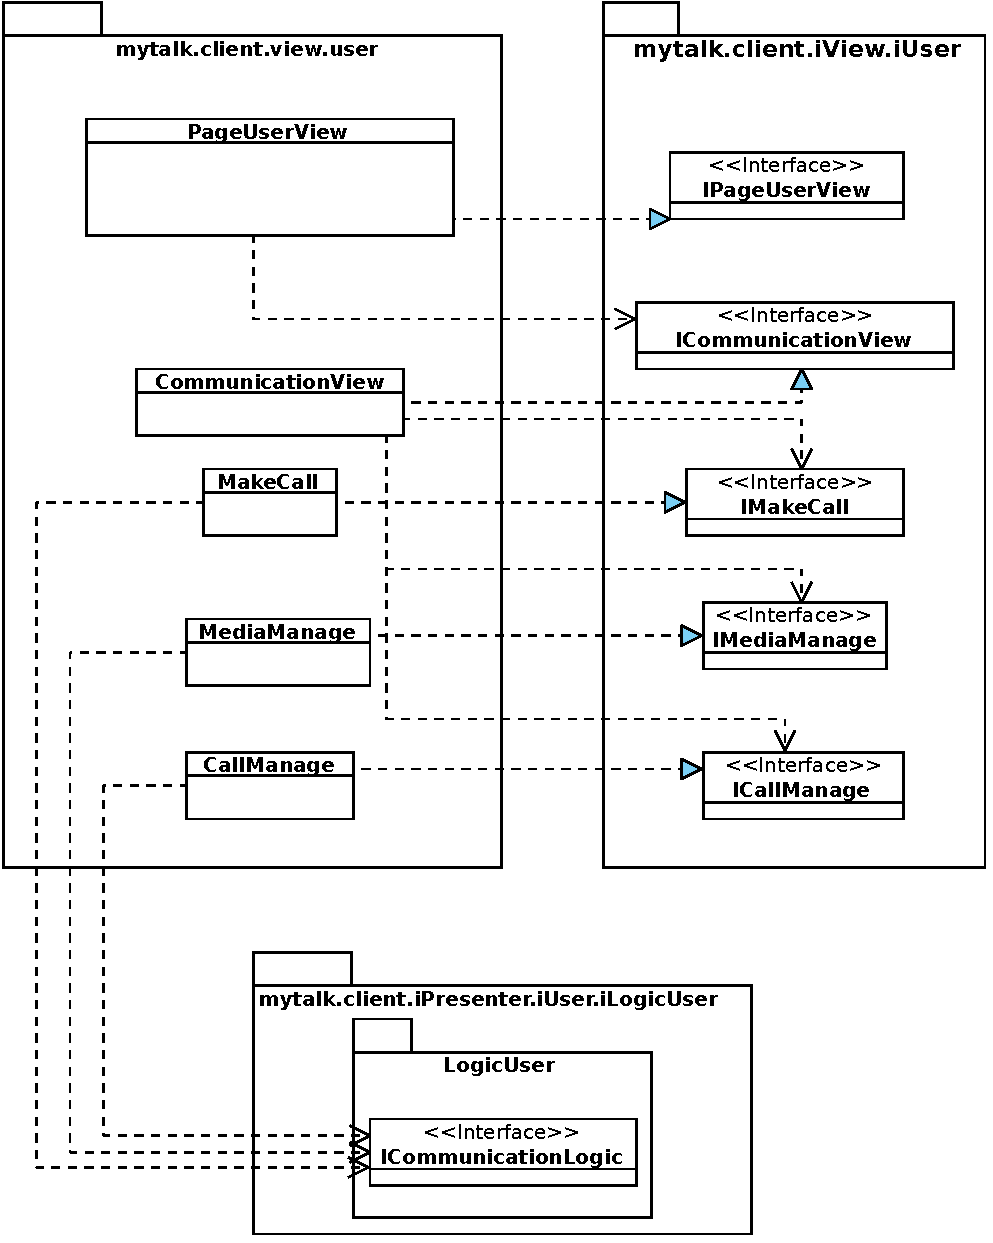
\includegraphics[scale=0.55]{\docsImg dia/MyTalk-View-User-com.pdf}
		\caption{Diagramma delle classi che illustra la View utente per la comunicazione.}
	\end{figure}

%interfacce
\paragraph{IPageUserView}{
	\begin{itemize}
		\item [] \textbf{Nome:} \texttt{IPageUserView}
		\item [] \textbf{Tipo:} interface
		\item [] \textbf{Package:} \texttt{mytalk.client.iView.iUser}
		\item [] \textbf{Descrizione:}{ interfaccia che permette di modificare la pagina dell'utente fruitore del servizio su richiesta del Presenter.}
	\end{itemize}
}
\paragraph{ILogUser}{
	\begin{itemize}
		\item [] \textbf{Nome:} \texttt{ILogUser}
		\item [] \textbf{Tipo:} interface
		\item [] \textbf{Package:} \texttt{mytalk.client.iView.iUser}
		\item [] \textbf{Descrizione:}{ interfaccia che permette di richiedere l'accesso o la terminazione dell'utente all'utilizzo del prodotto. Le classi che implementano questa interfaccia hanno il compito di raccogliere ed inoltrare al sottosistema Presenter i dati di accesso, nel caso di un login, e distruggere la sessione utente in caso di logout.}
	\end{itemize}
}
\paragraph{IRegister}{
	\begin{itemize}
		\item [] \textbf{Nome:} \texttt{IRegister}
		\item [] \textbf{Tipo:} interface
		\item [] \textbf{Package:} \texttt{mytalk.client.iView.iUser}
		\item [] \textbf{Descrizione:}{ interfaccia che rappresenta la richiesta di inserire i dati per la creazione di un nuovo utente. Le classi che implementano questa interfaccia hanno il compito di inviare i dati inseriti dall'utente al livello Presenter.}
	\end{itemize}
}
\paragraph{IUserDataView}{
	\begin{itemize}
		\item [] \textbf{Nome:} \texttt{IUserDataView}
		\item [] \textbf{Tipo:} interface
		\item [] \textbf{Package:} \texttt{mytalk.client.iView.iUser}
		\item [] \textbf{Descrizione:}{ interfaccia che permette all'utente di inviare al Presenter una richiesta per recuperare i propri dati e gestirli.}
	\end{itemize}
}
\paragraph{IShowDataUser}{
	\begin{itemize}
		\item [] \textbf{Nome:} \texttt{IShowDataUser}
		\item [] \textbf{Tipo:} interface
		\item [] \textbf{Package:} \texttt{mytalk.client.iView.iUser}
		\item [] \textbf{Descrizione:}{ interfaccia che rappresenta una richiesta di visualizzazione dei dati dell'utente selezionato. Le classi che implementano questa interfaccia hanno il compito di inviare al Presenter una richiesta di recupero dei dati dell'utente autenticato.}
	\end{itemize}
}
\paragraph{IModifyDataUser}{
	\begin{itemize}
		\item [] \textbf{Nome:} \texttt{IModifyDataUser}
		\item [] \textbf{Tipo:} interface
		\item [] \textbf{Package:} \texttt{mytalk.client.iView.iUser}
		\item [] \textbf{Descrizione:}{ interfaccia che permette di richiedere la modifica dei dati relativi all'utente selezionato. Le classi che implementano questa interfaccia hanno il compito di raccogliere i nuovi dati inseriti e di inviare una richiesta al Presenter che poi provvederà a modificarli.}
	\end{itemize}
}
\paragraph{ICommunicationView}{
	\begin{itemize}
		\item [] \textbf{Nome:} \texttt{ICommunicationView}
		\item [] \textbf{Tipo:} interface
		\item [] \textbf{Package:} \texttt{mytalk.client.iView.iUser}
		\item [] \textbf{Descrizione:}{ interfaccia che rappresenta la costruzione della GUI\g~ per la gestione della comunicazione da parte dell'utente attuale.}
	\end{itemize}
}
\paragraph{ICallManage}{
	\begin{itemize}
		\item [] \textbf{Nome:} \texttt{ICallManage}
		\item [] \textbf{Tipo:} interface
		\item [] \textbf{Package:} \texttt{mytalk.client.iView.iUser}
		\item [] \textbf{Descrizione:}{ interfaccia che rappresenta la gestione delle comunicazioni in atto o in entrata. Le classi che implementano questa interfaccia hanno il compito di inviare segnali al Presenter, su richiesta dell'utente, che permettono di gestire la comunicazione.}
	\end{itemize}
}
\paragraph{IMediaManage}{
	\begin{itemize}
		\item [] \textbf{Nome:} \texttt{IMediaManage}
		\item [] \textbf{Tipo:} interface
		\item [] \textbf{Package:} \texttt{mytalk.client.iView.iUser}
		\item [] \textbf{Descrizione:}{ le classi che implementano questa interfaccia hanno il compito di emettere opportuni segnali al Presenter, per la gestione dei media.}
	\end{itemize}
}
\paragraph{IMakeCall}{
	\begin{itemize}
		\item [] \textbf{Nome:} \texttt{IMakeCall}
		\item [] \textbf{Tipo:} interface
		\item [] \textbf{Package:} \texttt{mytalk.client.iView.iUser}
		\item [] \textbf{Descrizione:}{ interfaccia che permette di richiedere l'effettuazione di una nuova comunicazione dato un riferimento all'utente destinatario. Le classi che implementano questa interfaccia hanno il compito di inviare i dati di comunicazione al livello Presenter e mostrare lo stato della chiamata all'utente.}
	\end{itemize}
}
%classi
}
}
\subsection{Package mytalk.client.view}{

\subsubsection{Package mytalk.client.view.administrator}{

%classi
\paragraph{PageAdminView}{
	\begin{itemize}
		\item [] \textbf{Nome:} \texttt{PageAdminView}
		\item [] \textbf{Tipo:} class
		\item [] \textbf{Package:} \texttt{mytalk.client.view.administrator}
		\item [] \textbf{Descrizione:} la classe ha il compito di gestire la creazione dei widget\g~ che compongono l'interfaccia dell'amministratore su richiesta del Presenter.
		\item [] \textbf{Relazioni con altre componenti:} la classe implementa l'interfaccia\\ \texttt{mytalk.client.iView.iAdministrator.IPageAdminView}.\\
		Richiama inoltre metodi delle classi
\texttt{mytalk.client.view.administrator.LogAdminView}, \\
\texttt{mytalk.client.view.administrator.StatisticView} e \\
\texttt{mytalk.client.presenter.administrator.logicAdmin.UpdateViewLogic}.
	\end{itemize}
}
\paragraph{LogAdmin}{
	\begin{itemize}
		\item [] \textbf{Nome:} \texttt{LogAdmin}
		\item [] \textbf{Tipo:} class
		\item [] \textbf{Package:} \texttt{mytalk.client.view.administrator}
		\item [] \textbf{Descrizione:}{ la classe ha il compito di creare i widget\g~ che compongono la parte della pagina web\g~ che permette all'amministratore di autenticarsi e di uscire dal servizio. La classe ha anche il compito di dialogare con il Presenter per verificare la correttezza dei dati inseriti e per dargli istruzione di distruggere i dati della sessione.}
		\item [] \textbf{Relazioni con altre componenti:} la classe implementa l'interfaccia\\ \texttt{mytalk.client.iView.iAdministrator.ILogAdmin}\\ e fa parte per composizione della classe\\ \texttt{mytalk.client.view.administrator.PageAdminView}.\\
		Richiama inoltre metodi della classe\\ \texttt{mytalk.client.presenter.administrator.logicAdmin.LogAdminLogic}\\ per gestire gli eventi generati dall'utente.
	\end{itemize}
}
\paragraph{StatisticView}{
	\begin{itemize}
		\item [] \textbf{Nome:} \texttt{StatisticView}
		\item [] \textbf{Tipo:} class
		\item [] \textbf{Package:} \texttt{mytalk.client.view.administrator}
		\item [] \textbf{Descrizione:}{questa classe mette a disposizione dell'amministratore i widget\g~ che gli permettono di visualizzare e filtrare, tramite vari parametri, le statistiche inviate dagli utenti che hanno effettuato una comunicazione e che sono memorizzate nel sistema, la classe dialoga con il Presenter per richiedere le statistiche.}
		\item [] \textbf{Relazioni con altre componenti:}{ la classe implementa l'interfaccia\\ \texttt{mytalk.client.iView.iAdministrator.IStatisticView} e fa parte per composizione della classe \texttt{mytalk.client.view.administrator.PageAdminView}.\\ Richiama inoltre metodi della classe\\ \texttt{mytalk.client.presenter.administrator.logicAdmin.StatisticLogic}\\ per gestire gli eventi generati dall'utente.}
	\end{itemize}
}
}%admin


\subsubsection{Package mytalk.client.view.user}{
\paragraph{PageUserView}{
	\begin{itemize}
		\item [] \textbf{Nome:} \texttt{PageUserView}
		\item [] \textbf{Tipo:} class
		\item [] \textbf{Package:} \texttt{mytalk.client.view.user}
		\item [] \textbf{Descrizione:} la classe ha il compito di gestire la creazione dei widget\g, su richiesta del Presenter, che compongono l'interfaccia dell'utente, con le informazioni che il Presenter provvederà a fornire.
		\item [] \textbf{Relazioni con altre componenti:} la classe implementa l'interfaccia\\ \texttt{mytalk.client.iView.iUser.IPageUserView}.\\
		Richiama inoltre metodi delle classi \\
		\texttt{mytalk.client.view.user.LogUserView},
		\texttt{mytalk.client.view.user.RegisterView}, \\
		\texttt{mytalk.client.view.user.UserDataView}, \\
		\texttt{mytalk.client.view.user.CommunicationView}, \\
		\texttt{mytalk.client.presenter.user.logicUser.UpdateViewLogic} e \\
		\texttt{mytalk.client.presenter.user.logicUser.serverComUser.WebSocketUser}.
	\end{itemize}
}
\paragraph{LogUser}{
	\begin{itemize}
		\item [] \textbf{Nome:} \texttt{LogUser}
		\item [] \textbf{Tipo:} class
		\item [] \textbf{Package:} \texttt{mytalk.client.view.user}
		\item [] \textbf{Descrizione:} tale classe ha il compito di generare l'evento che permette al Presenter di gestire correttamente la fase di autenticazione al sistema, visualizzando eventualmente un output adeguato all'esito dell'operazione. La classe ha anche il compito di generare l'evento per l'uscita dal servizio.
		\item [] \textbf{Relazioni con altre componenti:} la classe implementa l'interfaccia\\ \texttt{mytalk.client.iView.iUser.ILogUser}.\\
		Richiama inoltre metodi delle classi \\
		\texttt{mytalk.client.presenter.user.logicUser.LogUserLogic} e \\ \texttt{mytalk.client.presenter.user.logicUser.UpdateViewLogic}
		per gestire gli eventi generati dall'utente.
	\end{itemize}
}
\paragraph{Register}{
	\begin{itemize}
		\item [] \textbf{Nome:} \texttt{Register}
		\item [] \textbf{Tipo:} class
		\item [] \textbf{Package:} \texttt{mytalk.client.view.user}
		\item [] \textbf{Descrizione:} la classe \texttt{mytalk.client.view.user.PageUserView}, su richiesta del Presenter visualizza all'utente un form dove egli potrà inserire i propri dati per la registrazione. Tali dati vengono passati al livello Presenter dalla classe Register, il Presenter effettuerà la registrazione al servizio qualora i dati siano corretti.
		\item [] \textbf{Relazioni con altre componenti:} la classe implementa l'interfaccia\\ \texttt{mytalk.client.iView.iUser.IRegister}.\\ Richiama inoltre metodi delle classi\\ \texttt{mytalk.client.presenter.user.logicUser.RegisterLogic} e \\
		\texttt{mytalk.client.presenter.user.logicUser.UpdateViewLogic} per gestire gli eventi generati dall'utente nella fase di registrazione.
	\end{itemize}
}
\paragraph{UserDataView}{
	\begin{itemize}
		\item [] \textbf{Nome:} \texttt{UserDataView}
		\item [] \textbf{Tipo:} class
		\item [] \textbf{Package:} \texttt{mytalk.client.view.user}
		\item [] \textbf{Descrizione:}questa classe ha il compito di gestire la visualizzazione e di mettere a disposizione le opportune form che l'utente può utilizzare per modificare i dati.
		\item [] \textbf{Relazioni con altre componenti:} la classe implementa l'interfaccia\\ \texttt{mytalk.client.iView.iUser.IUserDataView} ed e' composta da due oggetti, uno di tipo\\ \texttt{mytalk.client.view.user.ShowDataUser} e uno di tipo\\ \texttt{mytalk.client.view.user.ModifyDataUser}.\\
		Richiama inoltre metodi delle classi \\
		\texttt{mytalk.client.presenter.user.logicUser.DataUserLogic} e \\
		\texttt{mytalk.client.presenter.user.logicUser.UpdateViewLogic}
		per gestire gli eventi generati dall'utente ed aggiornare l'interfaccia.
	\end{itemize}
}
\paragraph{ShowDataUser}{
	\begin{itemize}
		\item [] \textbf{Nome:} \texttt{ShowDataUser}
		\item [] \textbf{Tipo:} class
		\item [] \textbf{Package:} \texttt{mytalk.client.view.user}
		\item [] \textbf{Descrizione:} tale classe ha la responsabilità di richiamare opportune funzioni del Presenter, che richiedono il reperimento delle informazioni personali dell'utente.
		\item [] \textbf{Relazioni con altre componenti:} la classe implementa l'interfaccia\\ \texttt{mytalk.client.iView.iUser.IShowDataUser}. Richiama inoltre metodi della classe\\ \texttt{mytalk.client.presenter.user.logicUser.DataUserLogic} per gestire gli eventi generati dall'utente, nella gestione del proprio account.
	\end{itemize}
}
\paragraph{ModifyDataUser}{
	\begin{itemize}
		\item [] \textbf{Nome:} \texttt{ModifyDataUser}
		\item [] \textbf{Tipo:} class
		\item [] \textbf{Package:} \texttt{mytalk.client.view.user}
		\item [] \textbf{Descrizione:} la classe ha il compito di permettere all'utente il cambiamento dei propri dati personali. La classe ha il compito di emettere eventi, su richiesta dell'utente, che richiedono al Presenter di modificare un certo dato.
		\item [] \textbf{Relazioni con altre componenti:} la classe implementa l'interfaccia\\ \texttt{mytalk.client.iView.iUser.IModifyDataUser}.
		Richiama inoltre metodi della classe \texttt{mytalk.client.presenter.user.logicUser.DataUserLogic} per gestire gli eventi generati dall'utente, nella gestione del proprio account.
	\end{itemize}
}
\paragraph{CommunicationView}{
	\begin{itemize}
		\item [] \textbf{Nome:} \texttt{CommunicationView}
		\item [] \textbf{Tipo:} class
		\item [] \textbf{Package:} \texttt{mytalk.client.view.user}
		\item [] \textbf{Descrizione:} la classe crea e distribuisce i vari widget\g~ nella pagina che consentono all'utente di comunicare, chiudere la comunicazione, visualizzare i media, inviare richieste di comunicazione ad altri utenti e chiudere le comunicazioni in atto.
		\item [] \textbf{Relazioni con altre componenti:} della classe fanno parte per composizione le classi \texttt{mytalk.client.view.user.MediaManage}, \texttt{mytalk.client.view.user.MakeCall},\\ \texttt{mytalk.client.view.user.CallManage}.\\
		Richiama inoltre metodi delle classi \\
		\texttt{mytalk.client.presenter.client.user.logicUser.CommunicationLogic}, \\
		\texttt{mytalk.client.view.user.MakeCall} e \\
		\texttt{mytalk.client.presenter.client.user.logicUser.UpdateViewLogic} per gestire l'interfaccia di comunicazione utente.
	\end{itemize}
}
\paragraph{CallManage}{
	\begin{itemize}
		\item [] \textbf{Nome:} \texttt{CallManage}
		\item [] \textbf{Tipo:} class
		\item [] \textbf{Package:} \texttt{mytalk.client.view.user}
		\item [] \textbf{Descrizione:} tale classe permette all'utente di gestire chiamate in arrivo, permettendo all'utente di accettare o rifiutare la chiamata. Nel caso la chiamata sia accettata, la classe invierà opportuna comunicazione al livello Presenter il quale provvederà ad instaurare la chiamata e ad aggiornare la GUI\g.
		\item [] \textbf{Relazioni con altre componenti:} la classe implementa l'interfaccia\\ \texttt{mytalk.client.iView.iUser.ICallManage}.\\
		Richiama inoltre metodi della classe \\ \texttt{mytalk.client.presenter.user.logicUser.CommunicationLogic} per gestire gli eventi generati dall'utente, nella gestione e/o instaurazione della chiamata.
	\end{itemize}
}
\paragraph{MediaManage}{
	\begin{itemize}
		\item [] \textbf{Nome:} \texttt{MediaManage}
		\item [] \textbf{Tipo:} class
		\item [] \textbf{Package:} \texttt{mytalk.client.view.user}
		\item [] \textbf{Descrizione:} la classe contiene i vari eventi generabili dall'utente che servono alla gestione dei media.
		\item [] \textbf{Relazioni con altre componenti:} la classe implementa l'interfaccia\\ \texttt{mytalk.client.iView.iUser.IMediaManage}.\\
		Richiama inoltre metodi della classe \\ \texttt{mytalk.client.presenter.user.logicUser.CommunicationLogic} per gestire gli eventi generati dall'utente, nella gestione e/o instaurazione della chiamata.
	\end{itemize}
}
\paragraph{MakeCall}{
	\begin{itemize}
		\item [] \textbf{Nome:} \texttt{MakeCall}
		\item [] \textbf{Tipo:} class
		\item [] \textbf{Package:} \texttt{mytalk.client.view.user}
		\item [] \textbf{Descrizione:} la classe permette all'utente di chiamare altri utenti, richiamando opportuni metodi del Presenter con i dati inseriti dall'utente.
		\item [] \textbf{Relazioni con altre componenti:} la classe implementa l'interfaccia\\ \texttt{mytalk.client.iView.iUser.IMakeCall}.\\
		Richiama inoltre metodi della classe \\ \texttt{mytalk.client.presenter.user.logicUser.CommunicationLogic} per gestire gli eventi generati dall'utente, nella gestione e/o instaurazione della chiamata.
	\end{itemize}
}
} %user
} %view





\newpage
\subsection{Package mytalk.client.iPresenter}

\subsubsection{Package mytalk.client.iPresenter.iAdministrator.iLogicAdmin}

\paragraph{ILogAdminLogic}{
	\begin{itemize}
		\item [] \textbf{Nome:} \texttt{ILogAdminLogic}
		\item [] \textbf{Tipo:} interface
		\item [] \textbf{Package:} \texttt{mytalk.client.iPresenter.iAdministrator.iLogicAdmin}
		\item [] \textbf{Descrizione:} { interfaccia che rappresenta l'accesso alle classi logiche che hanno il compito di gestire il login e logout dell'utente amministratore al servizio.}
	\end{itemize}
}
\paragraph{IStatisticLogic}{
	\begin{itemize}
		\item [] \textbf{Nome:} \texttt{IStatisticLogic}
		\item [] \textbf{Tipo:} interface
		\item [] \textbf{Package:} \texttt{mytalk.client.iPresenter.iAdministrator.iLogicAdmin}
		\item [] \textbf{Descrizione:}{ interfaccia che rappresenta l'accesso alle classi logiche che hanno il compito di recuperare ed elaborare i dati statistici delle chiamate effettuate.}
	\end{itemize}
}

\paragraph{IUpdateViewLogic}{
	\begin{itemize}
		\item [] \textbf{Nome:} \texttt{IUpdateViewLogic}
		\item [] \textbf{Tipo:} interface
		\item [] \textbf{Package:} \texttt{mytalk.client.iPresenter.iAdministrator.iLogicAdmin}
		\item [] \textbf{Descrizione:}{ interfaccia che fornisce le operazioni per aggiornare l'interfaccia grafica.}
	\end{itemize}
}
\subsubsection{Package mytalk.client.iPresenter.iAdministrator.iServerComAdmin}
\paragraph{IWebSocketAdmin}{
	\begin{itemize}
		\item [] \textbf{Nome:} \texttt{IWebSocketAdmin}
		\item [] \textbf{Tipo:} interface
		\item [] \textbf{Package:} \texttt{mytalk.client.iPresenter.iAdministrator.iServerComAdmin}
		\item [] \textbf{Descrizione:}{ interfaccia che rappresenta le classi logiche dell'amministratore che hanno il compito di formattare i dati delle altre classi per poi trasmetterli al server\g~ tramite WebSocket\g.}
	\end{itemize}
}

\subsubsection{Package mytalk.client.iPresenter.iUser.iLogicUser}

\begin{figure}[h!tbp]
		\centering
		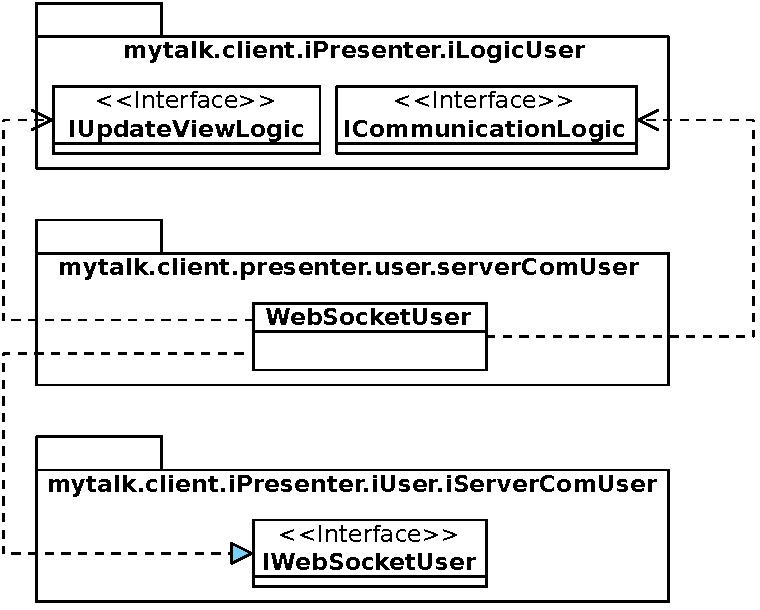
\includegraphics[scale=0.8]{\docsImg dia/MyTalk-Presenter-commUser.pdf}
		\caption{Diagramma delle classi che illustra il Presenter per l'operazione di comunicazione.}
	\end{figure}

%interfacce
\paragraph{ILogUserLogic}{
	\begin{itemize}
		\item [] \textbf{Nome:} \texttt{ILogUserLogic}
		\item [] \textbf{Tipo:} interface
		\item [] \textbf{Package:} \texttt{mytalk.client.iPresenter.iUser.iLogicUser}
		\item [] \textbf{Descrizione:}{ interfaccia che rappresenta l'accesso alle classi logiche che hanno il compito di gestire il login e logout dell'utente al servizio.}
	\end{itemize}
}
\paragraph{IRegisterLogic}{
	\begin{itemize}
		\item [] \textbf{Nome:} \texttt{IRegisterLogic}
		\item [] \textbf{Tipo:} interface
		\item [] \textbf{Package:} \texttt{mytalk.client.iPresenter.iUser.iLogicUser}
		\item [] \textbf{Descrizione:}{ interfaccia che rappresenta l'accesso alle classi logiche che hanno il compito di gestire i dati di registrazione inseriti dall'utente nella View.}
	\end{itemize}
}
\paragraph{IDataUserLogic}{
	\begin{itemize}
		\item [] \textbf{Nome:} \texttt{IDataUserLogic}
		\item [] \textbf{Tipo:} interface
		\item [] \textbf{Package:} \texttt{mytalk.client.iPresenter.iUser.iLogicUser}
		\item [] \textbf{Descrizione:}{ interfaccia che rappresenta l'accesso agli oggetti che gestiscono il recupero e la modifica, verificandone la conformità, dei dati propri dell'utente e inoltra le richieste di comunicazione alla componente dedita alla comunicazione con il server\g .}
	\end{itemize}
}
\paragraph{IUpdateViewLogic}{
	\begin{itemize}
		\item [] \textbf{Nome:} \texttt{IUpdateViewLogic}
		\item [] \textbf{Tipo:} interface
		\item [] \textbf{Package:} \texttt{mytalk.client.iPresenter.iUser.iLogicUser}
		\item [] \textbf{Descrizione:}{ interfaccia che fornisce le operazioni per aggiornare l'interfaccia grafica.}
	\end{itemize}
}
\paragraph{ICommunicationLogic}{
	\begin{itemize}
		\item [] \textbf{Nome:} \texttt{ICommunicationLogic}
		\item [] \textbf{Tipo:} interface
		\item [] \textbf{Package:} \texttt{mytalk.client.iPresenter.iUser.iLogicUser}
		\item [] \textbf{Descrizione:}{ interfaccia che rappresenta l'accesso alle classi che hanno il compito di comporre gli oggetti che serviranno per instaurare una nuova comunicazione, gestire le comunicazioni in ingresso e l'accesso ai media locali e remoti.}
	\end{itemize}
}



\subsubsection{Package mytalk.client.iPresenter.iUser.iCommunication}

\paragraph{IPeerConnection}{
	\begin{itemize}
		\item [] \textbf{Nome:} \texttt{IPeerConnection}
		\item [] \textbf{Tipo:} interface
		\item [] \textbf{Package:} \texttt{mytalk.client.iPresenter.iUser.iCommunication}
		\item [] \textbf{Descrizione:}{ interfaccia che fornisce le operazioni per la gestione della connessione peer-to-peer.}
	\end{itemize}
}
	
\paragraph{IMediaStream}{
	\begin{itemize}
		\item [] \textbf{Nome:} \texttt{IMediaStream}
		\item [] \textbf{Tipo:} interface
		\item [] \textbf{Package:} \texttt{mytalk.client.iPresenter.iUser.iCommunication}
		\item [] \textbf{Descrizione:}{ interfaccia che fornisce le operazioni per gestire ed ottenere i media locali.}
	\end{itemize}
}

\subsubsection{Package mytalk.client.iPresenter.iUser.iServerComUser}
\paragraph{IWebSocketUser}{
	\begin{itemize}
		\item [] \textbf{Nome:} \texttt{IWebSocketUser}
		\item [] \textbf{Tipo:} interface
		\item [] \textbf{Package:} \texttt{mytalk.client.iPresenter.iUser.iServerComUser}
		\item [] \textbf{Descrizione:}{ interfaccia che rappresenta le classi logiche dell'utente che hanno il compito di formattare i dati delle altre classi per poi trasmetterli al server\g~ tramite WebSocket\g.}
	\end{itemize}
}
\newpage

\subsection{Package mytalk.client.presenter}
\noindent Di seguito è riportata la descrizione delle classi per quanto concerne la parte del Presenter che risiede sul client\g .

	\begin{figure}[h!tbp]
		\centering
		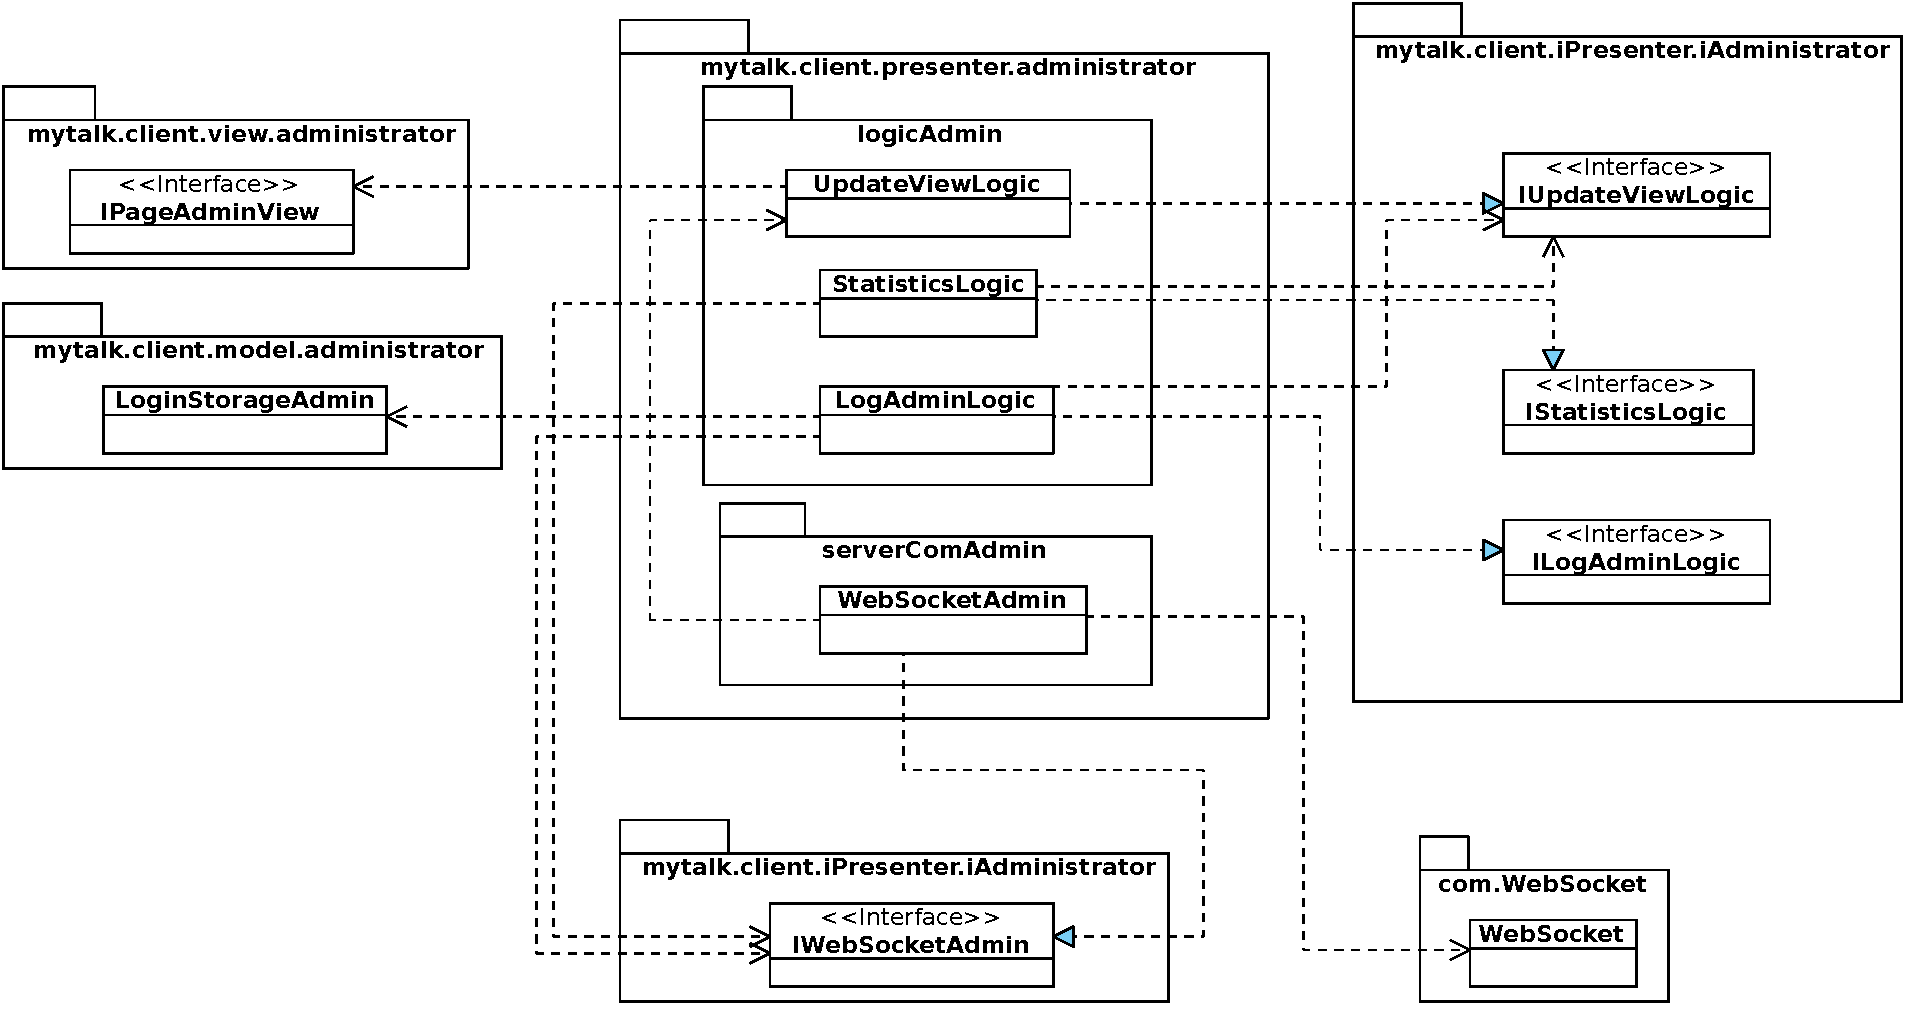
\includegraphics[scale=0.55]{\docsImg dia/MyTalk-Client-Presenter-Administrator.pdf}
		\caption{Diagramma delle classi che illustra il Presenter lato Client dell'administrator.}
	\end{figure}

\newpage

	\begin{figure}[h!tbp]
		\centering
		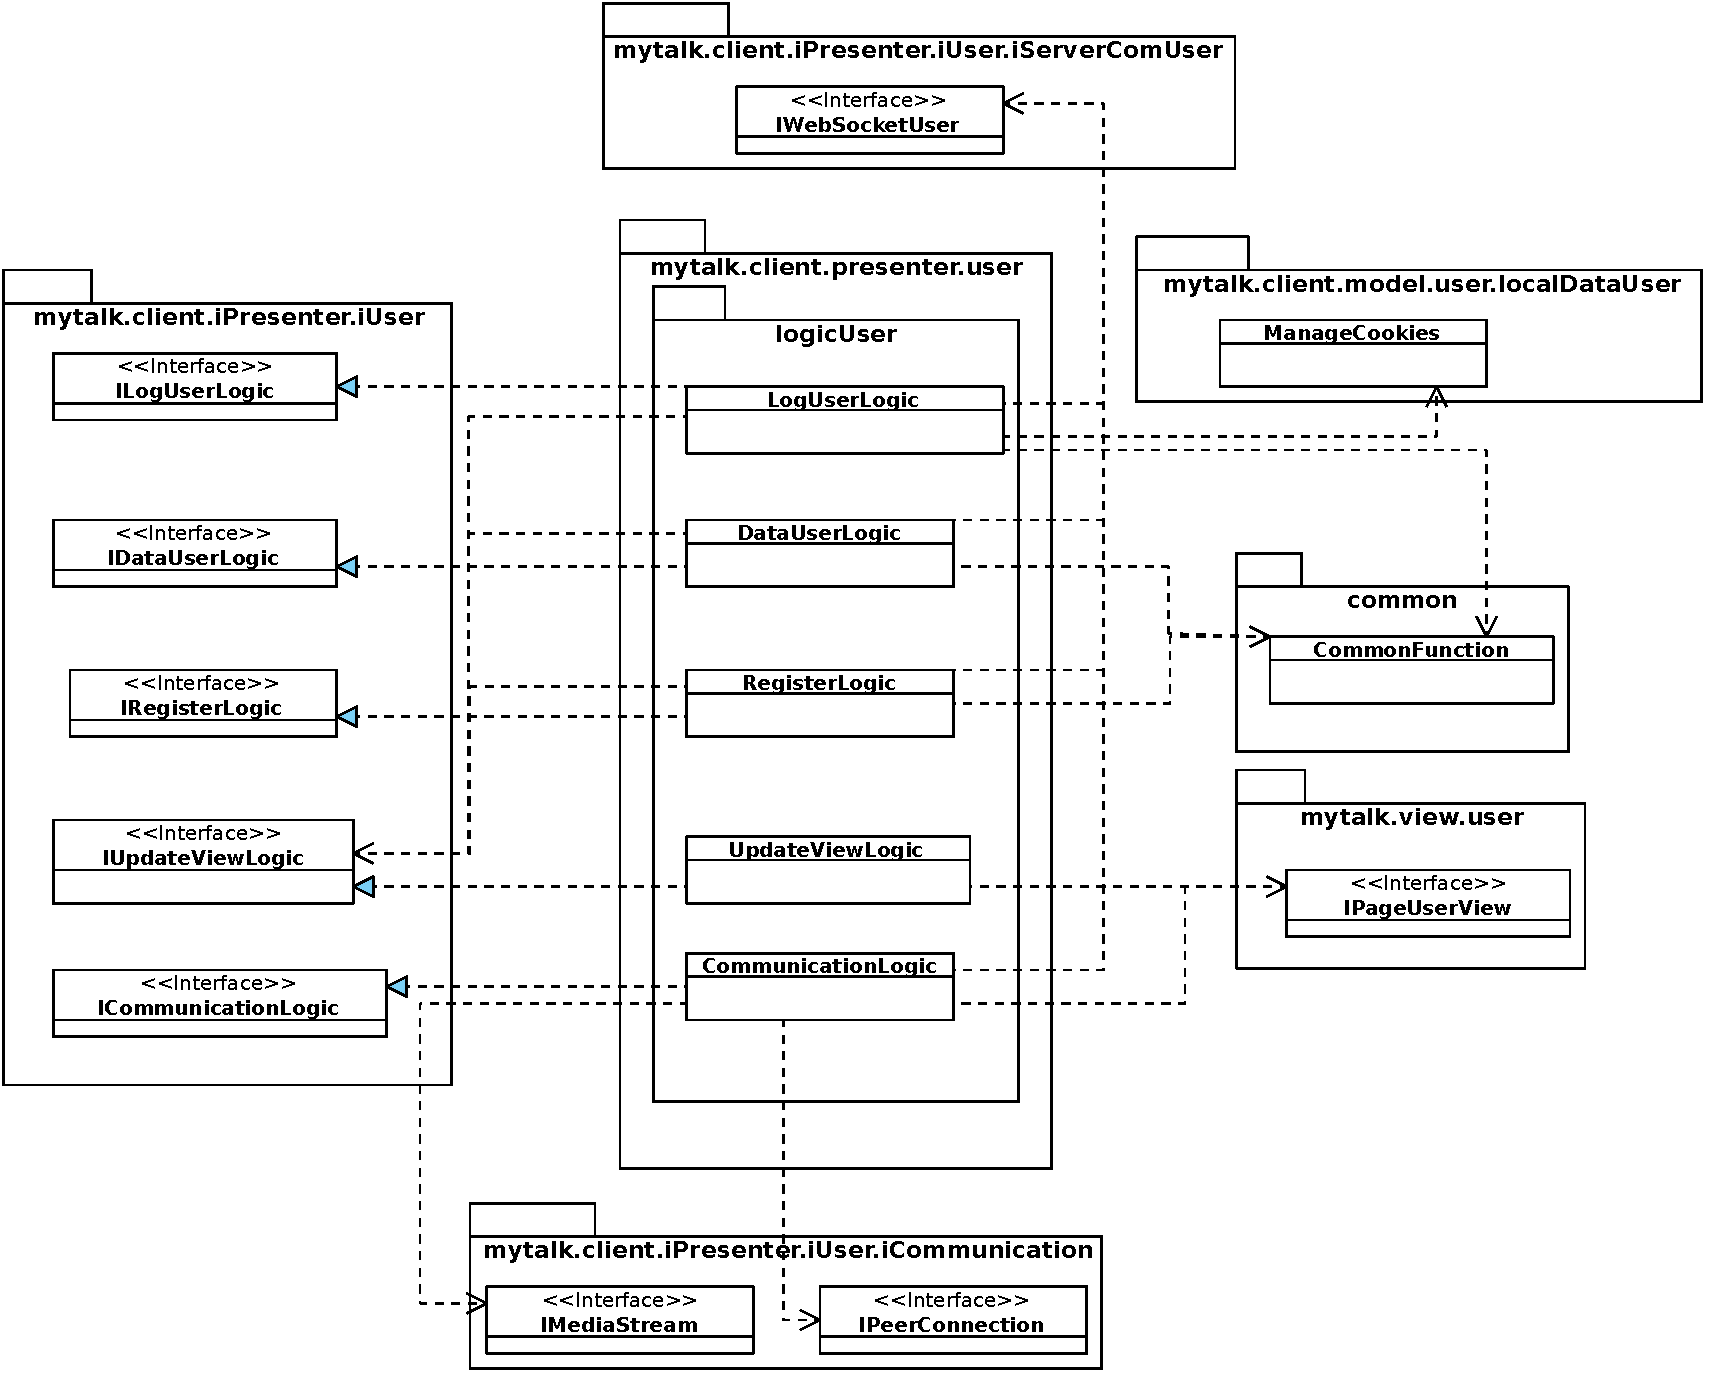
\includegraphics[scale=0.6]{\docsImg dia/MyTalk-Client-Presenter-User.pdf}
		\caption{Diagramma delle classi che illustra il Presenter lato Client dello user.}
	\end{figure}



\subsubsection{Package mytalk.client.presenter.administrator.logicAdmin}
%classi
\paragraph{LogAdminLogic}{
	\begin{itemize}
		\item [] \textbf{Nome:} \texttt{LogAdminLogic}
		\item [] \textbf{Tipo:} class
		\item [] \textbf{Package:} \texttt{mytalk.client.presenter.administrator.LogicAdmin}
		\item [] \textbf{Descrizione:}  questa classe ha il compito di gestire gli eventi provenienti dalla componente View, di accesso ed uscita dal servizio, in particolare dalla classe\\ \texttt{mytalk.client.view.administrator.LogAdmin}. La classe, dopo aver opportunamente gestito l'evento, ritorna un responso sull'esito dell'operazione alla View. Nel caso di login, il responso sarà o il reindirizzamento alla pagina principale (segno di autenticazione riuscita) o un opportuno messaggio che descrive la natura dell'errore avvenuto. Nel caso di logout, il responso sarà il reindirizzamento alla pagina di login.		
		\item [] \textbf{Relazioni con altre componenti:} implementa l'interfaccia\\ \texttt{mytalk.client.iPresenter.iAdministrator.iLogicAdmin.ILogAdminLogic}, richiama metodi delle classi \\
 \texttt{mytalk.client.presenter.administrator.serverComAdmin.WebSocketAdmin} e \\ \texttt{mytalk.client.presenter.user.logicUser.common.CommonFunctions} per inviare e ricevere messaggi dal server\g , comunica con la classe\\ \texttt{mytalk.client.presenter.administrator.logicAdmin.UpdateViewLogic}\\ per gestire l'aggiornamento della pagina e comunicare l'esito delle operazioni effettuate all'utente.
	\end{itemize}
}
\paragraph{StatisticLogic}{
	\begin{itemize}
		\item [] \textbf{Nome:} \texttt{StatisticLogic}
		\item [] \textbf{Tipo:} class
		\item [] \textbf{Package:} \texttt{mytalk.client.presenter.administrator.logicAdmin}
		\item [] \textbf{Descrizione:} questa classe deve poter gestire gli eventi generati dalla View dell'amministratore, in particolare dalla classe \\ \texttt{mytalk.client.view.administrator.StatisticView}, la quale è responsabile dell'invio degli eventi per la visualizzazione delle statistiche. La classe avrà il compito di reperire ed inviare alla View le statistiche raccolte dai vari client\g.
		\item [] \textbf{Relazioni con altre componenti:} implementa l'interfaccia\\ \texttt{mytalk.client.iPresenter.iAdministrator.iLogicAdmin.IStatisticsLogic}, richiama metodi delle classi \\ \texttt{mytalk.client.presenter.administrator.logicAdmin.UpdateViewLogic} e \\ \texttt{mytalk.client.presenter.administrator.logicAdmin.serverComAdmin.WebSocketAdmin} per inviare e ricevere messaggi dal server\g , comunica con la classe\\ \texttt{mytalk.client.presenter.administrator.logicAdmin.UpdateViewLogic}\\ per gestire l'aggiornamento della pagina e comunicare l'esito delle operazioni effettuate all'utente.
	\end{itemize}
}

\paragraph{UpdateViewLogic}{
	\begin{itemize}
		\item [] \textbf{Nome:} \texttt{UpdateViewLogic}
		\item [] \textbf{Tipo:} class
		\item [] \textbf{Package:} \texttt{mytalk.client.presenter.administrator.logicAdmin}
		\item [] \textbf{Descrizione:} la classe avrà il compito di aggiornare l'interfaccia grafica in seguito ad eventi generati da altre classi della componente Presenter.
		\item [] \textbf{Relazioni con altre componenti:} implementa l'interfaccia\\ \texttt{mytalk.client.iPresenter.iAdministrator.iLogicAdmin.IUpdateViewLogic}, richiama metodi della classe\\ \texttt{mytalk.client.view.administrator.logicAdmin.PageAdminView}\\ per gestire gli aggiornamenti dell'interfaccia grafica.
	\end{itemize}
}

\subsubsection{Package mytalk.client.presenter.administrator.logicAdmin.common}
\paragraph{CommonFunctions}{
	\begin{itemize}
		\item [] \textbf{Nome:} \texttt{CommonFunctions}
		\item [] \textbf{Tipo:} class
		\item [] \textbf{Package:} \texttt{mytalk.client.presenter.administrator.logicAdmin.common}
		\item [] \textbf{Descrizione:}{ classe che fornisce i metodi comuni a tutte le classi.}
	\end{itemize}
}


\subsubsection{Package mytalk.client.presenter.administrator.serverComAdmin}
\paragraph{WebSocketAdmin}{
	\begin{itemize}
		\item [] \textbf{Nome:} \texttt{WebSocketAdmin}
		\item [] \textbf{Tipo:} class
		\item [] \textbf{Package:} \texttt{mytalk.client.presenter.administrator.serverComAdmin}
		\item [] \textbf{Descrizione:}{ la classe permette di formattare i dati e le richieste degli amministratori per poi trasmetterli al server\g~ tramite WebSocket\g.}
		\item [] \textbf{Relazioni con altre componenti: } la classe implementa l'interfaccia\\ \texttt{mytalk.client.iPresenter.iAdministrator.iServerComAdmin.IWebSocketAdmin}, richiama metodi della classe\\ \texttt{mytalkadmin.client.presenter.logicAdmin.UpdateViewLogic}.
	\end{itemize}
}

\subsubsection{Package mytalk.client.presenter.user.serverComUser}

\paragraph{WebSocketUser}{
	\begin{itemize}
		\item [] \textbf{Nome:} \texttt{WebSocketUser}
		\item [] \textbf{Tipo:} class
		\item [] \textbf{Package:} \texttt{mytalk.client.presenter.user.serverComUser}
		\item [] \textbf{Descrizione:}{ la classe permette di formattare i dati e le richieste degli utenti per poi trasmetterli al server\g~ tramite WebSocket\g.}
		\item [] \textbf{Relazioni con altre componenti: } la classe implementa l'interfaccia \texttt{IWebSocketUser}, richiama metodi delle classi \texttt{com.WebSocket.WebSocket}, \\
		\texttt{mytalk.client.presenter.user.logicUser.CommunicationLogic}\\
		e \texttt{mytalk.client.presenter.user.logicUser.UpdateViewLogic} per gestire gli aggiornamenti dell'interfaccia grafica.
	\end{itemize}
}


\subsubsection{Package mytalk.client.presenter.user.logicUser}
%classi
\paragraph{LogUserLogic}{
	\begin{itemize}
		\item [] \textbf{Nome:} \texttt{LogUserLogic}
		\item [] \textbf{Tipo:} class
		\item [] \textbf{Package:} \texttt{mytalk.client.presenter.user.logicUser}
		\item [] \textbf{Descrizione:} questa classe ha il compito di gestire gli eventi provenienti dalla classe \texttt{mytalk.client.view.user.LogUser}. La classe ha quindi il compito di inoltrare la richiesta di login alla classe che ha il compito di comunicare con il server\g.
		La classe ha anche il compito di effettuare il logout dell'utente distruggendo i dati relativi alla sessione.
		\item [] \textbf{Relazioni con altre componenti:} la classe implementa l'interfaccia\\ \texttt{mytalk.client.iPresenter.iUser.iLogicUser.ILogUserLogic}, richiama metodi delle classi \texttt{mytalk.client.presenter.user.logicUser.common.CommonFunctions} e  \texttt{mytalk.client.presenter.user.logicUser.serverComUser.WebSocketUser}\\ per inviare e ricevere messaggi dal server\g, comunica con la classe\\ \texttt{mytalk.client.presenter.user.logicUser.UpdateViewLogic} per gestire l'aggiornamento della pagina e comunicare l'esito delle operazioni effettuate all'utente.
	\end{itemize}
}
\paragraph{RegisterLogic}{
	\begin{itemize}
		\item [] \textbf{Nome:} \texttt{RegisterLogic}
		\item [] \textbf{Tipo:} class
		\item [] \textbf{Package:} \texttt{mytalk.client.presenter.user.logicUser}
		\item [] \textbf{Descrizione:} la classe ha il compito di gestire gli eventi generati dalla classe \texttt{mytalk.client.view.Register}. La classe controlla i dati, dialogando con il server\g (tramite la classe \\ \texttt{mytalk.client.presenter.user.serverComUser.WebSocketUser}) e se questi risultano essere corretti procede con la registrazione e, successivamente, aggiorna la View (tramite la classe \texttt{mytalk.client.presenter.user.logicUser.UpdateViewLogic}). Altrimenti, riporta all'utente un opportuno messaggio per informarlo dell'errore.
		\item [] \textbf{Relazioni con altre componenti:} la classe implementa l'interfaccia\\ \texttt{mytalk.client.iPresenter.iUser.iLogicUser.IRegisterLogic}, richiama metodi delle classi \\ \texttt{mytalk.client.presenter.user.logicUser.common.CommonFunctions} e \\ \texttt{mytalk.client.presenter.user.serverComUser.WebSocketUser}\\ per inviare e ricevere messaggi dal server\g, comunica con la classe\\ \texttt{mytalk.client.presenter.user.logicUser.UpdateViewLogic}\\ per gestire l'aggiornamento della pagina e comunicare l'esito delle operazioni effettuate all'utente.
	\end{itemize}
}
\paragraph{DataUserLogic}{
	\begin{itemize}
		\item [] \textbf{Nome:} \texttt{DataUserLogic}
		\item [] \textbf{Tipo:} class
		\item [] \textbf{Package:} \texttt{mytalk.client.presenter.user.logicUser}
		\item [] \textbf{Descrizione:} tale classe ha il compito di ricevere e gestire gli eventi riguardanti la visualizzazione e la modifica di informazioni personali dell'utente provenienti dall'interfaccia grafica. Dopo aver ricevuto e gestito gli eventi, tale classe ha inoltre il compito di aggiornare l'interfaccia grafica con eventuali errori riscontrati nel controllo , mediante l'interfaccia\\ \texttt{mytalk.client.presenter.user.logicUser.UpdateViewLogic}.
		\item [] \textbf{Relazioni con altre componenti:} la classe implementa l'interfaccia\\ \texttt{mytalk.client.iPresenter.iUser.iLogicUser.IDataUserLogic},\\ richiama metodi della classe \\ \texttt{mytalk.client.presenter.user.serverComUser.WebSocketUser} per inviare e ricevere messaggi dal server\g, comunica con la classe\\ \texttt{mytalk.client.presenter.user.logicUser.UpdateViewLogic} per gestire l'aggiornamento della pagina e comunicare l'esito delle operazioni effettuate all'utente.
	\end{itemize}
}
\paragraph{UpdateViewLogic}{
	\begin{itemize}
		\item [] \textbf{Nome:} \texttt{UpdateViewLogic}
		\item [] \textbf{Tipo:} class
		\item [] \textbf{Package:} \texttt{mytalk.client.presenter.user.logicUser}
		\item [] \textbf{Descrizione:} la classe avrà il compito di aggiornare l'interfaccia grafica in seguito ad eventi generati da altre classi della componente Presenter.
		\item [] \textbf{Relazioni con altre componenti:} implementa l'interfaccia\\ \texttt{mytalk.client.iPresenter.iUser.iLogicUser.IUpdateViewLogic}, richiama metodi delle classi \texttt{mytalk.client.view.user.PageUserView},\\ \texttt{mytalk.client.presenter.user.logicUser.common.CommonFunction} e\\ \texttt{mytalk.client.presenter.user.serverComUser.WebSocketUser} per gestire gli aggiornamenti dell'interfaccia grafica.
	\end{itemize}
}
\paragraph{CommunicationLogic}{
	\begin{itemize}
		\item [] \textbf{Nome:} \texttt{CommunicationLogic}
		\item [] \textbf{Tipo:} class
		\item [] \textbf{Package:} \texttt{mytalk.client.presenter.user.logicUser}
		\item [] \textbf{Descrizione:} tale classe ha il compito di gestire gli eventi provenienti dalla classe \texttt{mytalk.client.view.user.CommunicationView}. Gli eventi che gestisce questa classe sono quindi quelli che riguardano la comunicazione: effettuare e ricevere chiamate e gestione degli stream\g~ audio e video.
		La classe, dopo aver ricevuto i dati dalla componente Model, aggiorna opportunamente la View visualizzando eventuali messaggi per l'utente ed aggiornando gli stream\g, il tutto tramite l'interfaccia \texttt{mytalk.client.view.user.IPageUserView}.
		\item [] \textbf{Relazioni con altre componenti:} implementa l'interfaccia\\ \texttt{mytalk.client.iPresenter.iUser.iLogicUser.ICommunicationLogic},\\ richiama metodi delle classi\\ \texttt{mytalk.client.presenter.user.communication.PeerConnection},\\  \texttt{mytalk.client.presenter.user.communication.MediaStream}\\ tramite le interfacce:\\ \texttt{mytalk.client.iPresenter.iUser.iCommunicaton.IPeerConnection},\\  \texttt{mytalk.client.iPresenter.iUser.iCommunication.IMediaStream}\\
		per poter stabilire  e gestire il canale di comunicazione.\\
		Richiama inoltre metodi della classe\\ \texttt{mytalk.client.presenter.user.serverComUser.WebSocketUser}\\ per inviare e ricevere messaggi dal server\g~ e comunica con la classe\\ \texttt{mytalk.client.presenter.user.logicUser.UpdateViewLogic}\\ per gestire l'aggiornamento della pagina e comunicare l'esito delle operazioni effettuate all'utente.
	\end{itemize}
}
\subsubsection{Package mytalk.client.presenter.user.logicUser.common}
\paragraph{CommonFunctions}{
	\begin{itemize}
		\item [] \textbf{Nome:} \texttt{CommonFunctions}
		\item [] \textbf{Tipo:} class
		\item [] \textbf{Package:} \texttt{mytalk.client.presenter.user.logicUser.common}
		\item [] \textbf{Descrizione:}{ classe che fornisce i metodi comuni a tutte le classi.}
	\end{itemize}
}
\subsubsection{Package mytalk.client.presenter.user.communication}
\paragraph{PeerConnection}{
	\begin{itemize}
		\item [] \textbf{Nome:} \texttt{PeerConnection}
		\item [] \textbf{Tipo:} class
		\item [] \textbf{Package:} \texttt{mytalk.client.presenter.user.communication}
		\item [] \textbf{Descrizione:} tale classe è la componente adapter del design pattern Adapter. Ha il compito di gestire la comunicazione peer-to-peer\g. Questo è reso possibile tramite la componente adaptee che è la classe WebRTCAdaptee che contiene le librerie WebRTC\g.
		\item [] \textbf{Relazioni con altre componenti:} implementa l'interfaccia\\ \texttt{mytalk.client.iPresenter.iUser.iCommunication.IPeerConnection}, richiama metodi della classe\\ \texttt{com.webrtc.WebRTCAdaptee}.
	\end{itemize}
}

\paragraph{MediaStream}{
	\begin{itemize}
		\item [] \textbf{Nome:} \texttt{MediaStream}
		\item [] \textbf{Tipo:} class
		\item [] \textbf{Package:} \texttt{mytalk.client.presenter.user.communication}
		\item [] \textbf{Descrizione: }tale classe è la componente adapter del design pattern Adapter. Ha il compito di gestire le informazioni riguardanti gli stream\g~ audio e video che permettono agli utenti di comunicare. Questo è reso possibile tramite la componente adaptee che è la classe MediaStream delle librerie getUserMedia\g.
		\item [] \textbf{Relazioni con altre componenti:} implementa l'interfaccia\\ \texttt{mytalk.client.presenter.iUser.iCommunication.IMediaStream} e richiama metodi delle API \texttt{getUserMedia}.
	\end{itemize}
}

\subsubsection{com.webrtc}
\paragraph{WebRTCAdaptee}{
	\begin{itemize}
		\item [] \textbf{Nome:} \texttt{WebRTCAdaptee}
		\item [] \textbf{Tipo:} class
		\item [] \textbf{Package:} \texttt{com.webrtc}
		\item [] \textbf{Descrizione:} tale classe è la componente adaptee del design pattern Adapter. Ha il compito di gestire la comunicazione peer-to-peer\g. 
		\item [] \textbf{Relazioni con altre componenti:} è utilizzata dalla classe\\ \texttt{mytalk.client.presenter.user.communication.PeerConnection}.
	\end{itemize}
}

\subsubsection{com.WebSocket}
\paragraph{WebSocket}{
	\begin{itemize}
		\item [] \textbf{Nome:} \texttt{WebSocket}
		\item [] \textbf{Tipo:} class
		\item [] \textbf{Package:} \texttt{com.WebSocket}
		\item [] \textbf{Descrizione:} tale classe è il webSocket\g~ che ha il compito di trasmettere e di ricevere i dati al server\g.
	\end{itemize}
}


\paragraph{MediaStream}{
	\begin{itemize}
		\item [] \textbf{Nome:} \texttt{MediaStream}
		\item [] \textbf{Tipo:} class
		\item [] \textbf{Package:} \texttt{com.WebRTC}
		\item [] \textbf{Descrizione:} tale classe è la componente adaptee del design pattern Adapter. Ha il compito di contenere e gestire le informazioni relative ai media di un peer\g~ e fa parte delle API \texttt{getUserMedia}.
		\item [] \textbf{Relazioni con altre componenti:} è utilizzata dalla classe\\ \texttt{mytalk.client.presenter.user.communication.MediaStream}.
	\end{itemize}
}

\newpage

\subsection{Package mytalk.server.presenter}
\noindent Di seguito è riportata la descrizione delle classi per quanto concerne la parte del Presenter che risiede sul server\g .

	\begin{figure}[h!tbp]
		\centering
		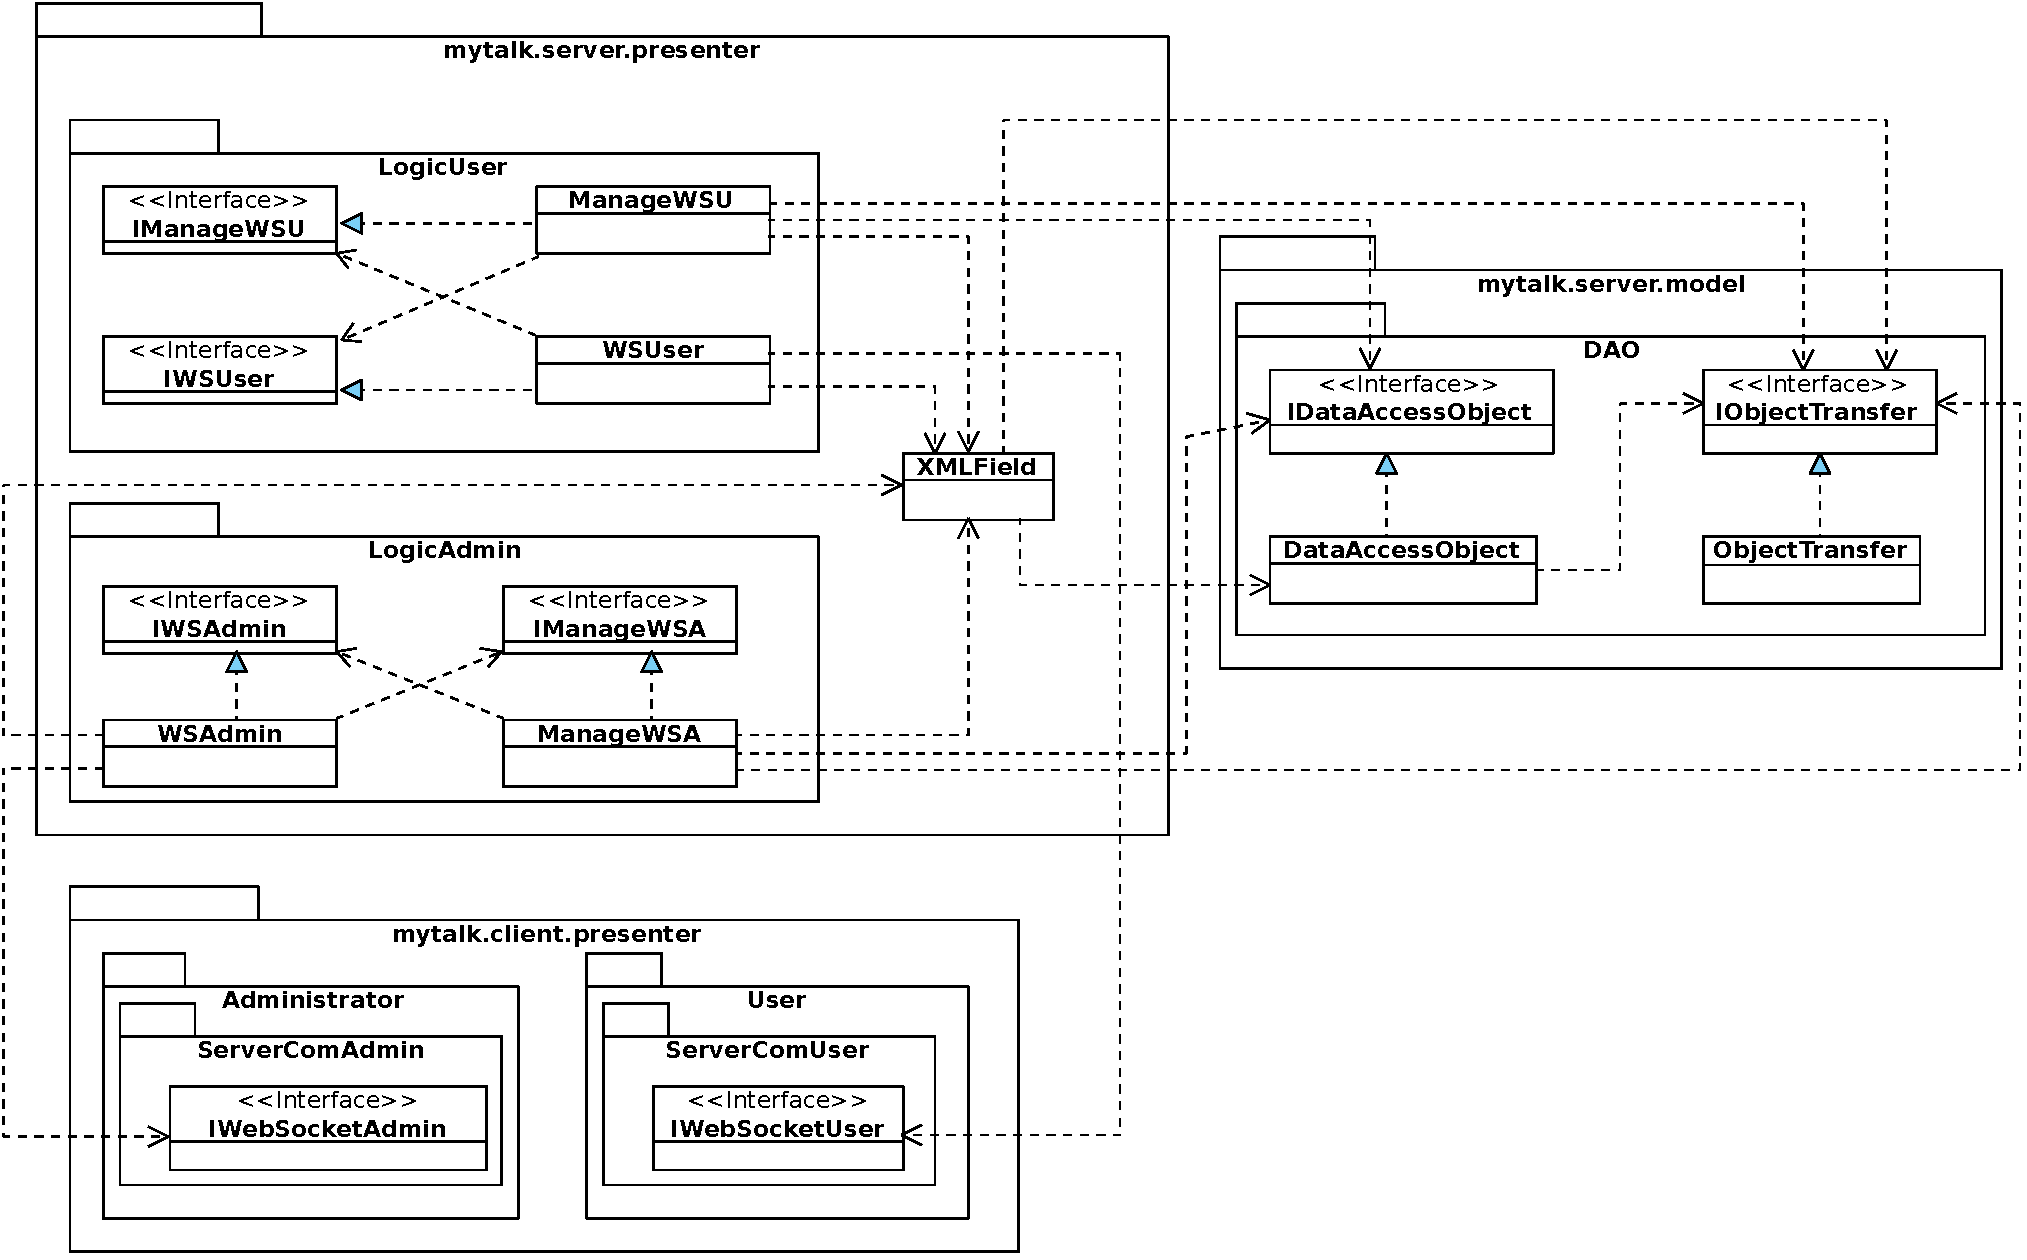
\includegraphics[scale=0.5]{\docsImg dia/MyTalk-Presenter-Server.pdf}
		\caption{Diagramma delle classi che illustra il Presenter lato server\g~.}
	\end{figure}

\subsubsection{Package mytalk.server.presenter}
\paragraph{XMLField}{
	\begin{itemize}
		\item [] \textbf{Nome:} \texttt{XMLField}
		\item [] \textbf{Tipo:} class
		\item [] \textbf{Package:} \texttt{mytalk.server.presenter}
		\item [] \textbf{Descrizione:}{ la classe che raccoglie i metodi comuni dei package\g~ \\ \texttt{mytalk.server.presenter.user.logicUser} e \\ \texttt{mytalk.server.presenter.administrator.logicAdmin} per gestione dei messaggi XML\g.
		}
	\end{itemize}
}

\newpage

\subsubsection{Package mytalk.server.presenter.user.logicUser}
\paragraph{IManageWSU}{
	\begin{itemize}
		\item [] \textbf{Nome:} \texttt{IManageWSU}
		\item [] \textbf{Tipo:} interface
		\item [] \textbf{Package:} \texttt{mytalk.server.presenter.user.logicUser}
		\item [] \textbf{Descrizione:}{ interfaccia che rappresenta la classe contenitrice delle connessioni WebSocket\g~ dal server\g~ verso il client\g, per quanto riguarda gli utenti. Le classi che la implementano devono gestire l'inoltro delle richieste di comunicazione agli utenti destinatari ed eventualmente comunicare con il Model.}
	\end{itemize}
}
\paragraph{IWSUser}{
	\begin{itemize}
		\item [] \textbf{Nome:} \texttt{IWSUser}
		\item [] \textbf{Tipo:} interface
		\item [] \textbf{Package:} \texttt{mytalk.server.presenter.user.logicUser}
		\item [] \textbf{Descrizione:}{ interfaccia pubblica della classe che gestisce il collegamento, tramite WebSocket\g, dal server\g al client\g per l'utente.}
	\end{itemize}
}

%classi
\paragraph{ManageWSU}{
	\begin{itemize}
		\item [] \textbf{Nome:} \texttt{ManageWSU}
		\item [] \textbf{Tipo:} class
		\item [] \textbf{Package:} \texttt{mytalk.server.presenter.user.logicUser}
		\item [] \textbf{Descrizione:} la classe ha il compito di gestire le richieste di comunicazione tra il server\g e il client\g degli utenti.\\ La comunicazione tra questi due livelli deve avvenire tramite WebSocket\g~. La classe dopo aver ricevuto un messaggio dalla classe che contiene il WebSocket\g, dovrà soddisfare la richiesta che è contenuta nel messaggio; eventualmente interrogando il Model o girando il messaggio verso un altro utente.
		\item [] \textbf{Relazioni con altre componenti:} la classe implementa l'interfaccia\\ \texttt{mytalk.server.presenter.user.logicUser.IManageWSU} e richiama metodi delle classi\\ \texttt{mytalk.server.model.dao.DataAccessObject} (tramite l'interfaccia\\ \texttt{mytalk.server.model.dao.IDataAccessObject}), \\ \texttt{mytalk.server.model.dao.ObjectTranfer} (tramite l'interfaccia\\ \texttt{mytalk.server.model.dao.IObjectTranfer}) e\\ \texttt{mytalk.server.presenter.XMLField} per interagire con la base di dati, dalla quale riceve, nel caso di restituzione di un risultato, oggetti di tipo\\ \texttt{mytalk.server.model.dao.ObjectTransfer}.
	\end{itemize}
}
\paragraph{WSUser}{
	\begin{itemize}
		\item [] \textbf{Nome:} \texttt{WSUser}
		\item [] \textbf{Tipo:} class
		\item [] \textbf{Package:} \texttt{mytalk.server.presenter.user.logicUser}
		\item [] \textbf{Descrizione:} la classe che gestisce il collegamento tramite WebSocket\g~ all'utente. Tale classe, oltre a ricevere la richiesta dal livello Presenter del client\g~ gira tale richiesta dopo averla tradotta in una opportuna chiamata di funzione alla sua classe contenitrice che è\\ \texttt{mytalk.server.presenter.user.logicUser}.
		\item [] \textbf{Relazioni con altre componenti:} la classe implementa l'interfaccia\\ \texttt{mytalk.server.presenter.user.logicUser.IWSUser} e richiama metodi della classe \texttt{mytalk.server.presenter.user.logicUser.ManageWSU}.
	\end{itemize}
}
\subsubsection{Package mytalk.server.presenter.administrator.logicAdmin}
\paragraph{IManageWSA}{
	\begin{itemize}
		\item [] \textbf{Nome:} \texttt{IManageWSA}
		\item [] \textbf{Tipo:} interface
		\item [] \textbf{Package:} \texttt{mytalk.server.presenter.administrator.logicAdmin}
		\item [] \textbf{Descrizione:}{ interfaccia che rappresenta la classe contenitrice delle connessioni WebSocket\g~ dal server\g~ verso il client\g, per quanto riguarda gli amministratori. Le classi che la implementano devono gestire l'inoltro delle richieste di interrogazione della base di dati da parte degli amministratori e le richieste di autenticazione.}
	\end{itemize}
}

\paragraph{IWSAdmin}{
	\begin{itemize}
		\item [] \textbf{Nome:} \texttt{IWSAdmin}
		\item [] \textbf{Tipo:} interface
		\item [] \textbf{Package:} \texttt{mytalk.server.presenter.administrator.logicAdmin}
		\item [] \textbf{Descrizione:}{ interfaccia pubblica della classe che gestisce il collegamento dal server\g verso il client\g, tramite WebSocket\g.}
	\end{itemize}
}

\paragraph{ManageWSA}{
	\begin{itemize}
		\item [] \textbf{Nome:} \texttt{ManageWSA}
		\item [] \textbf{Tipo:} class
		\item [] \textbf{Package:} \texttt{mytalk.server.presenter.administrator.logicAdmin}
		\item [] \textbf{Descrizione:} la classe ha il compito di ricevere, gestire e soddisfare le richieste che arrivano dal livello Presenter del client\g~ della componente amministratore. Tale classe, per soddisfare le richieste, effettua delle interazioni con la classe che interfaccia il database\g.
		\item [] \textbf{Relazioni con altre componenti:} la classe implementa l'interfaccia\\ \texttt{mytalk.server.presenter.logicAdmin.IManageWSA} e richiama metodi della classe\\ \texttt{mytalk.server.model.dao.DataAccessObject} (tramite l'interfaccia\\ \texttt{mytalk.server.model.dao.IDataAccessObject}), \\ \texttt{mytalk.server.model.dao.ObjectTranfer} (tramite l'interfaccia\\ \texttt{mytalk.server.model.dao.IObjectTranfer}) e\\ \texttt{mytalk.server.presenter.XMLField} per interagire con la base di dati, dalla quale riceve, nel caso di restituzione di un risultato, oggetti di tipo \\ \texttt{mytalk.server.model.dao.ObjectTransfer}.
	\end{itemize}
}
\paragraph{WSAdmin}{
	\begin{itemize}
		\item [] \textbf{Nome:} \texttt{WSAdmin}
		\item [] \textbf{Tipo:} class
		\item [] \textbf{Package:} \texttt{mytalk.server.presenter.logicAdmin}
		\item [] \textbf{Descrizione:} la classe che gestisce il collegamento tramite WebSocket\g~ all'utente amministratore. Tale classe, oltre a ricevere, soddisfa la richiesta del livello Presenter che può riguardare operazioni di autenticazione o visualizzazione delle statistiche.
		\item [] \textbf{Relazioni con altre componenti:} la classe implementa l'interfaccia\\ \texttt{mytalk.server.presenter.administrator.logicAdmin.IWSAdmin} ed utilizza i metodi definiti nella classe\\ \texttt{mytalk.server.presenter.administrator.logicAdmin.ManageWSA} tramite la sua interfaccia\\ \texttt{mytalk.server.presenter.administrator.logicAdmin.IManageWSA}. I metodi della classe vengono richiamati da tutti gli oggetti del Presenter.
	\end{itemize}
}


\subsection{Package mytalk.client.model}
\noindent Diseguito è riportata la descrizione delle componenti del Model che risiedono sul client\g.

	\begin{figure}[h!tbp]
		\centering
		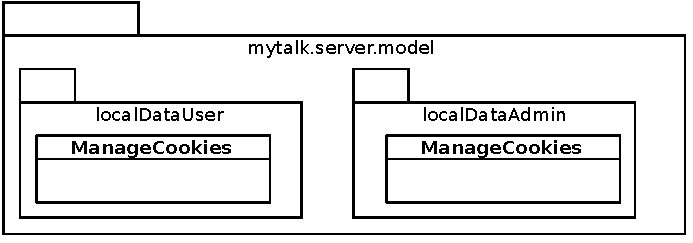
\includegraphics[scale=1]{\docsImg dia/MyTalk-Model-Client.pdf}
		\caption{Diagramma delle classi che illustra il Model lato Client.}
	\end{figure}

\subsubsection{Package mytalk.client.model.localDataAdmin}

\paragraph{ManageCookies}{
	\begin{itemize}
		\item [] \textbf{Nome:} \texttt{ManageCookies}
		\item [] \textbf{Tipo:} class
		\item [] \textbf{Package:} \texttt{mytalk.client.model.localDataAdmin}
		\item [] \textbf{Descrizione:}{ classe che rappresenta le informazioni di sessione salvate sul client\g~, tali informazioni riguardano l'amministratore attualmente autenticato, se questo esiste.}
	\end{itemize}
}

\subsubsection{Package mytalk.client.model.localDataUser}

\paragraph{ManageCookies}{
	\begin{itemize}
		\item [] \textbf{Nome:} \texttt{ManageCookies}
		\item [] \textbf{Tipo:} class
		\item [] \textbf{Package:} \texttt{mytalk.client.model.localDataUser}
		\item [] \textbf{Descrizione:}{ classe che rappresenta le informazioni di sessione salvate sul client\g, tali informazioni riguardano l'utente attualmente autenticato, se questo esiste.}
	\end{itemize}
}

\subsection{Package mytalk.server.model.dao}

	\begin{figure}[h!tbp]
		\centering
		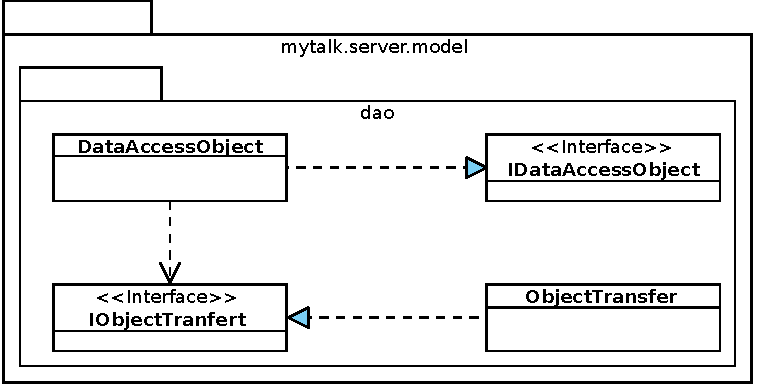
\includegraphics[scale=1]{\docsImg dia/MyTalk-Model-Server.pdf}
		\caption{Diagramma delle classi che illustra il Model lato Client.}
	\end{figure}

%interfacce
\paragraph{IDataAccessObject}{
	\begin{itemize}
		\item [] \textbf{Nome:} \texttt{IDataAccessObject}
		\item [] \textbf{Tipo:} interface
		\item [] \textbf{Package:} \texttt{mytalk.server.model.dao}
		\item [] \textbf{Descrizione:}{ interfaccia che rappresenta la connessione verso il database\g~ MySQL per il recupero e l'inserimento delle informazioni degli utenti.}
	\end{itemize}
}

\paragraph{IObjectTransfer}{
	\begin{itemize}
		\item [] \textbf{Nome:} \texttt{IObjectTransfer}
		\item [] \textbf{Tipo:} interface
		\item [] \textbf{Package:} \texttt{mytalk.server.model.dao}
		\item [] \textbf{Descrizione:}{ interfaccia che fornisce le operazioni per la gestione delle informazioni reperite o inserite nel DBMS\g.}
	\end{itemize}
}

\paragraph{DataAccessObject}{
	\begin{itemize}
		\item [] \textbf{Nome:} \texttt{DataAccessObject}
		\item [] \textbf{Tipo:} class
		\item [] \textbf{Package:} \texttt{mytalk.server.model.dao}
		\item [] \textbf{Descrizione:} la classe ha il compito di interfacciare il server\g~ con il database\g~ MySQL, nel quale risiedono i dati relativi agli utenti, agli amministratori e alle statistiche. La classe fa parte del design pattern DAO (Data Access Object) e qualora debba restituire un risultato lo farà restituendo un oggetto di tipo\\ \texttt{mytalk.server.model.dao.ObjectTransfer}, disaccoppiando in questo modo il resto dell'applicazione dalla base di dati sottostante.
		\item [] \textbf{Relazioni con altre componenti:} la classe implementa l'interfaccia\\ \texttt{mytalk.server.model.IDataAccessObject} ed utilizza i metodi definiti nella classe \texttt{mytalk.server.model.dao.ObjectTransfer} tramite la sua interfaccia  \texttt{mytalk.server.model.dao.IObjectTransfer}.
	\end{itemize}
}

\paragraph{ObjectTransfer}{
	\begin{itemize}
		\item [] \textbf{Nome:} \texttt{ObjectTransfer}
		\item [] \textbf{Tipo:} class
		\item [] \textbf{Package:} \texttt{mytalk.server.model.dao}
		\item [] \textbf{Descrizione:}{ questo oggetto rappresenta il tipo generico dell'oggetto che incapsulerà le informazioni restituite da una interrogazione al database.}
		\item [] \textbf{Relazioni con altre componenti:} la classe implementa l'interfaccia\\ \texttt{mytalk.server.model.IObjectTransfer}.
	\end{itemize}
}
